% !TeX spellcheck = de_DE
\documentclass{alex_gp}

\name{Alexander Helbok}
\course{Grundpraktikum}
\hwnumber{Fehlerrechnung}


\begin{document}
\renewcommand{\labelenumi}{\alph{enumi})}


\begin{mybox}{Richtiges Runden}
	\centering \( x = 1.2736 \unit{m};\qquad \alpha_x = 0.25034 \unit{m} \)
	\tcblower
	\begin{enumerate}
		\item \( \left(1.274 \pm 0.250 \right) \unit{m} \qquad \xmark \)  Nur eine signifikante Stelle im Fehler
	\tcbline
		\item \( \left(1.3 \pm 0.3 \right) \qquad \xmark \)  Keine Einheiten!
	\tcbline
		\item \( 1273 \pm 250 \unit{mm} \qquad \xmark \)  Nur eine signifikante Stelle im Fehler
	\tcbline
		\item \( 1.3(3) \unit{m} \qquad \cmark \)
	\tcbline
		\item \( 1.3(25) \unit{m} \qquad \xmark \)  Nur eine signifikante Stelle im Fehler
	\tcbline
		\item \(  (1.3 \pm 0.25034) \unit{m} \qquad \xmark \)  Nur eine signifikante Stelle im Fehler
	\end{enumerate}
\end{mybox}

\begin{mybox}{Fehlerfortpflanzung}
	\centering \( x = (17.4 \pm 0.3) \unit{V};\quad y = (9.3 \pm 0.7) \unit{V} \)
	\tcblower
	\begin{enumerate}
		\item \( z = x - y = 8.1(8) \unit{V} \)
	\tcbline
		\item \( z = 12x + 3y = 237(4) \unit{V} \)
	\tcbline
		\item \( z = 5xy = 8.1(6) \cdot 10^{2} \unit{V^2} \)
	\tcbline
		\item \( z = \tfrac{y^3}{x^2} = 2.7(6) \unit{V} \)
	\tcbline
		\item \( z = x^2 + 3y^2 = 5.6(4) \cdot 10^{2} \unit{V^2}\)
	\tcbline
		\item \( z = \arcsin(\tfrac{y}{x}) = 0.56(5) \)
	\tcbline
		\item \( z = \sqrt{3xy} = 22.0(9) \unit{V} \)
	\tcbline
		\item \( z = \ln(\tfrac{y}{x}) = -0.63(8) \)
	\tcbline
		\item \( z = \tfrac{x}{y^2} + \tfrac{y}{x^2} = 0.23(3) \unit{1/V} \)
	\tcbline
		\item \( z = 2\sqrt{\tfrac{y}{x}} = 1.46(6) \)
	\end{enumerate}
\end{mybox}

\begin{mybox}{Beispiel: Bestimmung der Fallbeschleunigung \( g \)}
	\begin{align*}
		&x_1 = 5.000(1) \unit{m};\quad &x_2 &= 17.000(1) \unit{m};\quad &t_x &= 77283.5(1) \unit{\micro\s} &&\\
		&z_1 = 0 \unit{m};\quad &z_2 &= 20.000(1) \unit{m};\quad &t_z &= 129335.3(1) \unit{\micro\s} &&
	\end{align*} 
	\tcblower
	\begin{enumerate}
		\item \( v = \tfrac{x_2 - x_1}{t_x} = 155.27(2) \unit{\v} \)
	\tcbline
		\item \( x(t) = x_0 + v_0t + \tfrac{1}{2}a_0t^2 \)
		\begin{flalign*}
			x(t_z) - x(0) &= (z_2 - z_1) + vt_z + \tfrac{1}{2}gt_z^2 &&\\[2ex]
			g &= 2\tfrac{(z_2 - z_1) - vt_z}{t_z^2} = -9.8(3) \unit{\a} &&
		\end{flalign*}
	\tcbline
		\item Das Experiment misst die Erdbeschleunigung \( g \) zwar etwas ungenau, das Ergebnis verträgt sich aber gut mit dem Literaturwert. Um die Unsicherheit in \( g \) zu vermindern, müsste man in genauere Distanzmessungen, da die Unsicherheiten in \( x_1, x_2 \) über \( 99 \% \) des Gesamtfehlers in \( v \) und \( \approx 85 \% \) in \( g \) ausmachen. Die Zeit hingegen trägt bei beiden Ergebnissen weniger als \( 1 \) Prozent bei und ist daher verhältnismäßig sehr genau.
	\end{enumerate}
\end{mybox}

\begin{mybox}{Plotten von Daten mit linearem Fit}
	\centering \[ \chi^2 = \sum_{i}^{N} \tfrac{\left(y_i - y(x_i)\right)^2}{\sigma_i^2} = \sum_{i}^{N} \tfrac{\left(y_i - ax_i - b \right)^2}{\sigma_i^2} \]
	\tcblower
	\begin{enumerate}
		\item 
		\begin{flalign*}
			\pdv{\chi^2}{a} &= \sum_{i}^{N} x_i \tfrac{\left(y_i - ax_i - b \right)^2}{\sigma_i^2} = 0 &&\\
			\pdv{\chi^2}{b} &= \sum_{i}^{N} \tfrac{\left(y_i - ax_i - b \right)^2}{\sigma_i^2} = 0 &&
		\end{flalign*}
		\begin{flalign}
			\label{eqn:a}
			a = \frac{N\sum_{i}x_iy_i - \sum_{i}x_i \sum_{i}y_i}{N\sum_{i}x_i^2 - \left(\sum_{i}x_i\right)^2};\quad 
			b = \frac{\sum_{i}x_i^2 \sum_{i}y_i - \sum_{i}x_i \sum_{i}x_iy_i}{N\sum_{i}x_i^2 - \left(\sum_{i}x_i\right)^2} &&
		\end{flalign}
	\tcbline
		\item 
		\begin{flalign*}
			a &\approx 0.034 &&\\
			b &\approx 0.086 &&
		\end{flalign*}
	\tcbline
		\item \(  \)
		\begin{figure}[H]
%			\vspace{-0.5cm}		
			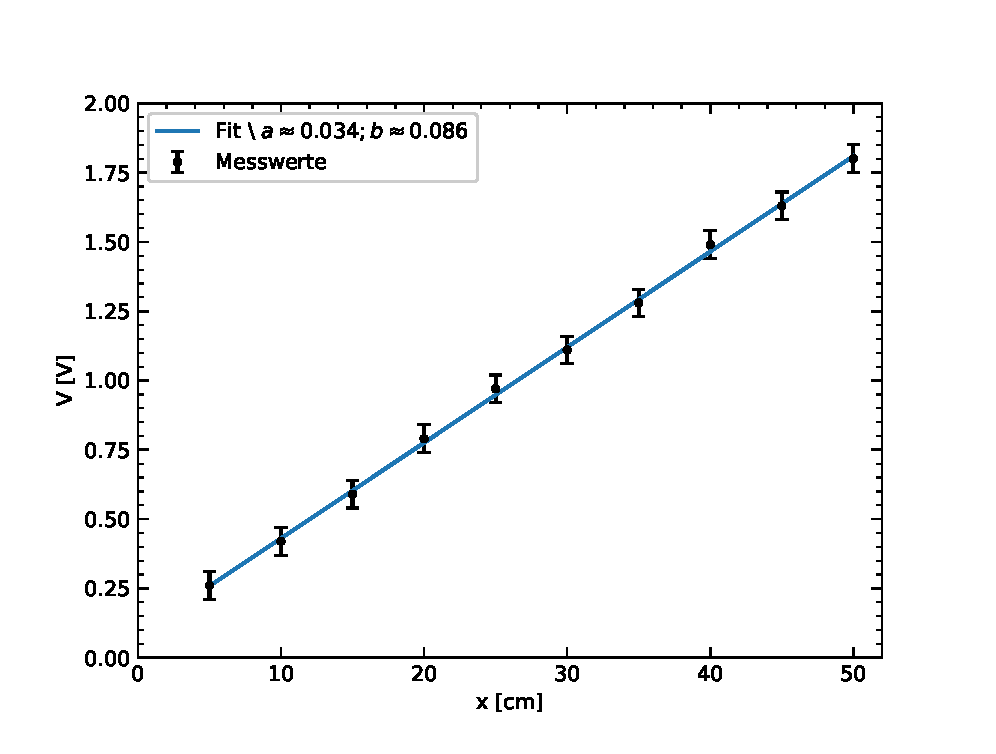
\includegraphics[width=\textwidth]{Fehlerrechnung_1.eps}
			\caption{Die Spannung an verschiedenen Orten gemessen. Die Fehlerbalken stellen einen \( 1 \sigma \) Standardfehler dar. Zudem wurde eine Gerade angepasst.}
		\end{figure}
		Die von SciPy berechnete Fitparameter stimmen den manuell berechneten überein, was andeutet, dass das Fitprogramm die gleiche Formel verwendet.
	\tcbline
		\item
		\begin{flalign*}
			\alpha_a &=  &&\\
			\alpha_b &=  &&
		\end{flalign*}
	\tcbline
		\item
		\begin{flalign*}
			\alpha_a &= 0.0011 &&\\
			\alpha_b &= 0.034 &&
		\end{flalign*}
		Die Fehler stimmen wieder überein, was die Hypothese unterstützt, dass das Fitprogramm von Gleichungen \ref{eqn:a} gebrauch macht.
	\tcbline
		\item Man könnte die Fitparameter \( a, b \) für \( x = \bar{x} - \alpha_x, x = \bar{x} \) und \( x = \bar{x} + \alpha_x \) mit Gleichungen \ref{eqn:a} berechnen und so Werte für \( \bar{a}, \bar{b}, \alpha_a, \alpha_b \) ermitteln. \par
		Alternativ könnte man bootstrapping verwenden, also aus dem Datensatz viele synthetische Datensätze (ohne Fehler) durch „ziehen mit zurücklegen“ zu generieren und auf diese die bekannten Formeln anwenden. Unter Annahme einer Normalverteilung kann man dann Mittelwert und Standardabweichung für die Fitparameter berechnen.
	\end{enumerate}
\end{mybox}

\begin{mybox}{Korrelierte Variablen}
	\centering \( y = ax + b;\quad a = 3.77;\quad b = 1.58;\quad \sigma = 
	\begin{pmatrix}
		0.033 & 0.019 \\
		0.019 & 0.009
	\end{pmatrix} \)
	\tcblower
	\begin{flalign*}
		y &= 0 \qquad \Rightarrow\qquad x = -\tfrac{b}{a} &&
	\end{flalign*}
\end{mybox}
	
\end{document}